%&pdflatex
\documentclass[12pt]{article}


\usepackage{graphicx}
\usepackage{colortbl}
\usepackage{xr}
\usepackage{longtable}
\usepackage{xfrac}
\usepackage{tabularx}
\usepackage{booktabs}
\usepackage{hyperref}
\usepackage{xcolor} % for different colour comments
\usepackage{fullpage}
\newcounter{rowcount}
\setcounter{rowcount}{0}
\usepackage{tikz}
\usetikzlibrary{shapes,arrows}


%% Diagram formatting
\tikzstyle{block} = [draw, fill=blue!20, rectangle, minimum height=3em, minimum
width=6em, text centered]
\tikzstyle{line} = [draw, -stealth', thick]
\tikzstyle{block2} = [draw, fill=blue!20, rectangle, minimum height=1em, minimum
width=2em, text centered]
\tikzstyle{arrow} = [thick,-,>=stealth]
\tikzstyle{arrow1} = [thick,->,>=stealth]
\tikzstyle{block3} = [draw, draw=black, fill=orange!20, rectangle, minimum
height=3em, minimum width=6em, text centered]


\hypersetup{
    bookmarks=true,         % show bookmarks bar?
    colorlinks=true,        % false: boxed links; true: colored links
    linkcolor=black,        % color of internal links (change box color with linkbordercolor)
    citecolor=green,        % color of links to bibliography
    filecolor=magenta,      % color of file links
    urlcolor=cyan           % color of external links
}

%% Comments
\newif\ifcomments\commentstrue
\ifcomments
\newcommand{\authornote}[3]{\textcolor{#1}{[#3 ---#2]}}
\newcommand{\todo}[1]{\textcolor{red}{[TODO: #1]}}
\else
\newcommand{\authornote}[3]{}
\newcommand{\todo}[1]{}
\fi
\newcommand{\wss}[1]{\authornote{magenta}{SS}{#1}}
\newcommand{\ds}[1]{\authornote{blue}{DS}{#1}}
\newcommand{\kly}[1]{\authornote{green}{KL}{#1}}
\newcommand{\cc}[1]{\authornote{orange}{CC}{#1}}

%%%%%%%%%%%%%%%%%%%%%%%%%%%%%

\begin{document}

\title{Design Document for Quarters}
\author{Team 6\\ \\James Anthony (anthonjb)\\ Wenqiang Chen (chenw25)\\ Carolyn Chong
(chongce)\\ Kevin Ly (lyk2)}
\date{\today}

\maketitle

\pagebreak

\tableofcontents

\section*{Revision History}
\begin{tabular}{|c|c|}
\hline
\textbf{Date}  & \textbf{Comments} \\ \hline
January 5, 2016 & Created first draft. \\
\hline
\end{tabular}

\pagebreak

%%%%%%%%%%%%%%%%%%%%%%%%%%%%%

%Introduction and Overview
\section{Introduction and Overview}

\subsection{Document Structure}
This document provides insight as to how Quarters was built. Design principles are stated followed by a list of anticipated and unlikely changes. The web application's system architecture is then decomposed and the design details explained based on the Software Requirements Specifications (SRS) document. Lastly, error handling is discussed and a project schedule is presented.

\subsection{Design Principles}
TBC. includes a clear statement of what design principle(s) is (are)being used. The web application was designed in a XXX manner. This was to ensure XXX. Decomposition follows the design principle suggested for the design. In many cases the appropriate design principle will be design for change (information hiding). Methodologies include top-down, bottom-up, stepwise refinement, prototyping, modular, or object-oriented.


%Connection between requirements and design
\section{Connection between requirements and design}
what design decisions needed to be made torealize the requirements – for instance, if there are security NFRs, what decision is made onhow to do this – password protection?

%Anticipated Changes
\section{Anticipated Changes}
\begin{enumerate}
\item{}
\end{enumerate}

%System Tests
\section{Unlikely Changes}
\begin{enumerate}
\item{}
\end{enumerate}

%
\section{Decomposition into Components}

%
\section{Uses hierarchy, or control flow diagram, or inheritance graph}

%
\section{Traceability from requirements to design components}

%
\section{Traceability for anticipated changes to components}

%
\section{Error Handling}

%
\section{User interface elements descriptions}
A description of the user interface design of Quarters is presented here. This section is divided into subsections of the UI navigation flow and the major UI elements. Each UI element is explained with the support of screen images and mockups.

\subsection{Navigation Flow}
See Figure 1.

\begin{figure}
\centering
\begin{tikzpicture}[auto, node distance=3.5cm]

% Place nodes
\node [block](bulletin){Bulletin Board};
\node [block, above of=bulletin](login){Login};
\node [block, left of=login](signup){Sign Up};
\node [block, above of=signup](landing){Landing Page};
\node [block, below of=bulletin, xshift=-7cm](house){House Settings};
\node [block, right of=house](calendar){Calendar};
\node [block, right of=calendar](messages){Messages};
\node [block, right of=messages](finances){Finances};
\node [block, right of=finances](maintenance){Maintenance};

% Place lines
\draw [arrow1] (landing) -- (signup);
\draw [arrow1] (signup) -- (login);
\draw [arrow1] (login) -- (bulletin);
\draw [arrow] (bulletin.south) -- ++(0,0) -- ++(0,-1) -| (house.north);
\draw [arrow] (bulletin.south) -- ++(0,0) -- ++(0,-1) -| (calendar.north);
\draw [arrow] (bulletin.south) -- ++(0,0) -- ++(0,-1) -| (messages.north);
\draw [arrow] (bulletin.south) -- ++(0,0) -- ++(0,-1) -| (finances.north);
\draw [arrow] (bulletin.south) -- ++(0,0) -- ++(0,-1) -| (maintenance.north);

\end{tikzpicture}
\caption{Quarters UI Navigation Flow Diagram}
\end{figure}

\subsection{Landing Page}
New users are directed to the landing page. The landing page provides information about the web application's features, and allows the potential user to sign up. There is also a login button for returning users. Both the signup and login buttons are placed in convenient and discoverable locations. The landing page is designed to capture a potential user's interest in the web application by making it appear modern, secure, easy to use, and beneficial through the use of fonts, colors, and layout. A big image covers the landing page that is meant to evoke feelings for a desire of that lifestyle the user could have if they joined Quarters.

\subsection{Sign Up}
The sign up page is designed to be simple and straightforward to allow for a quick process.

\subsection{Login}
The login page is designed to be simple and straightforward to allow for a quick process.

\subsection{Bulletin Board}
The bulletin board (bulletin for convenience) is the main page of the application. From here, every other page can be accessed via the navigation bar. Every user's bulletin is personalized based on their activity. Posts are the focus of this page and are listed in chronological order to be intuitive. Each post is listed with a corresponding icon that symbolizes the type of activity. A large box is positioned at the top of the bulletin to allow users to share content quickly. \\

\noindent Every page of the application has the same layout. There is a top navigation bar, and left navigation bar, and a large space to hold the content of that specific page. The structure of the navigation bars are consistent throughout the application to improve learnability. Fonts, colors and layout are consistent, as well. The whole application experience, from signing up to logging out, is mobile friendly. This means that regardless of screen window size, the user will be able to access all functionality of the application. For example, the navigation bars are collapsed to a toggle menu in smaller screen sizes to ensure the screen real estate is occupied mainly by content that the user will spend the most time looking at.

\subsection{House Settings}
House settings can be accessed from the bulletin. Documents, members and details about the creation of the house are included here. The interface of this section should simple and uncluttered.

\subsection{Calendar}
The Calendar resembles the UI of the Google Calendar because it is a widely used calendar that allows for some familiarity. A check list tab is easily accessible to change the visibility of different calendars. Buttons to add events are positioned above the Calendar.

\subsection{Messages}
A simple chat history of direct messages between two users is displayed here. The messages section is separate from the online users section. An image of the user accompanies each message. Again, a simple, uncluttered interface is important to ensure the user experience is as quick as possible.

\subsection{Finances}
The main focus of this page is a table displaying all bills.

\subsection{Maintenance}
This section holds a list of maintenance tickets in chronological order. Each ticket is accompanied by a corresponding icon to symbolize the type of ticket. Colors are used to differentiate the priority levels of each ticket. Each ticket is its own horizontal panel.

%
\section{Overview of key algorithms}

\clearpage
%
\section{Relational database structure}
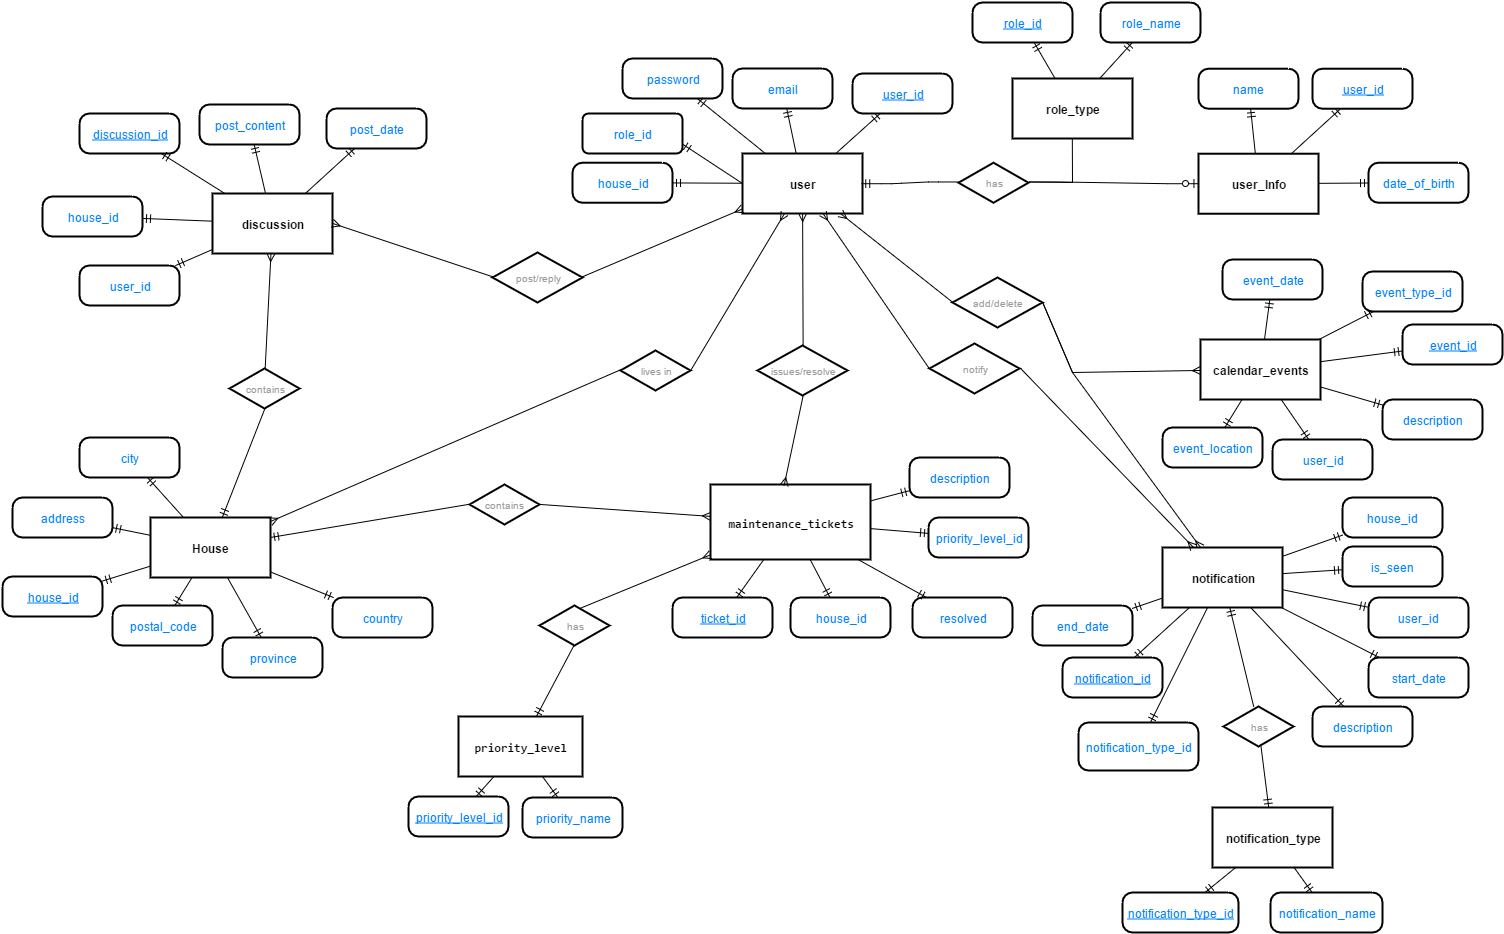
\includegraphics[scale=0.397, angle=-90, keepaspectratio]{images/ER_Diagram.png}
%
\section{Communication protocols specified}

%
\section{Description of each component, or UI element, or database table}

%
\section{Development Details}
\begin{description}
  \item[Languages of implementation] \hfill
    \begin{itemize}
      \item \href{https://nodejs.org/en/}{NodeJS}
      \item \href{http://www.postgresql.org/}{PostgreSQL}
      \item \href{http://jade-lang.com/}{Jade}
    \end{itemize}
  \item[Supporting frameworks] \hfill
    \begin{itemize}
      \item \href{http://getbootstrap.com/}{Bootstrap}
      \item \href{http://expressjs.com/}{ExpressJS}
    \end{itemize}
  \item[Supporting technology] \hfill
    \begin{itemize}
      \item \href{http://www.ubuntu.com/server}{Ubuntu Server}
    \end{itemize}
\end{description}
%
\section{GanttProject shows a detailed project schedule}

%
\section{Pert chart shows dependencies}

\end{document}
